\documentclass[11pt]{article}

\usepackage{amsmath}
\usepackage{amssymb}
\usepackage{graphicx}
\usepackage{booktabs}
\usepackage{hyperref}

\title{An Example Paper}
\author{Your Name\\Your Institution}
\date{\today}

\begin{document}
\maketitle

\begin{abstract}
This example shows the parts of a typical research paper: sections kept in
separate files, an equation, a figure, a table, cross-references and a
bibliography. Replace the text with your own and keep the structure you need.
\end{abstract}

\section{Introduction}
\label{sec:introduction}

\TeX{} was designed for typesetting text with a lot of mathematics~\cite{knuth1984texbook},
and \LaTeX{} adds the document structure most papers rely on~\cite{lamport1994latex}.
Section~\ref{sec:method} describes the method, Section~\ref{sec:results} reports the
results, and Section~\ref{sec:conclusion} concludes.

\section{Method}
\label{sec:method}

We model the quantity of interest as the mean of $n$ observations
$x_1, \dots, x_n \in \mathbb{R}$:
\begin{equation}
  \bar{x} = \frac{1}{n} \sum_{i=1}^{n} x_i .
  \label{eq:mean}
\end{equation}
Equation~\eqref{eq:mean} is used for every measurement in Section~\ref{sec:results}.

\section{Results}
\label{sec:results}

Figure~\ref{fig:example} shows the mean from Equation~\eqref{eq:mean} for five runs,
and Table~\ref{tab:results} lists the same values.

\begin{figure}[htbp]
  \centering
  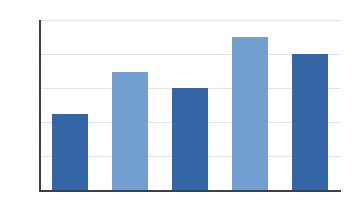
\includegraphics[width=0.6\linewidth]{figures/example-figure.png}
  \caption{Mean value per run.}
  \label{fig:example}
\end{figure}

\begin{table}[htbp]
  \centering
  \caption{Mean value per run.}
  \label{tab:results}
  \begin{tabular}{lr}
    \toprule
    Run & Mean \\
    \midrule
    1 & 0.45 \\
    2 & 0.70 \\
    3 & 0.60 \\
    4 & 0.90 \\
    5 & 0.80 \\
    \bottomrule
  \end{tabular}
\end{table}

\section{Conclusion}
\label{sec:conclusion}

We summarised the method of Section~\ref{sec:method} and the results in
Table~\ref{tab:results}. For more on structuring long documents, see
\cite{mittelbach2004companion}.


\bibliographystyle{plain}
\bibliography{references}

\end{document}
